\documentclass{article}
\usepackage[serbian]{babel}
\usepackage{cmsrb}
\usepackage[OT2,T1]{fontenc}
\usepackage{hyperref}
\usepackage{amsmath}
\usepackage{graphicx}
\usepackage{hyperref}
\hypersetup{
    colorlinks,
    citecolor=black,
    filecolor=black,
    linkcolor=blue,
    urlcolor=blue
}

\begin{document}

\fontencoding{OT2}\selectfont

\title{{\huge {\fontencoding{T1}\selectfont Fuzzy} klasterovanje}}

\author{Maja Crnomarkovi\'{c} 21/2017\\Marko Babi\'{c} 77/2017}
\date{25. jun 2021.}

\maketitle

\centerline{{\normalsize Seminarski rad u okviru kursa}}
\centerline{{\normalsize Ra\v{c}unarska inteligencija}}

\begin{figure}[h]
\vspace{1cm}
\centerline{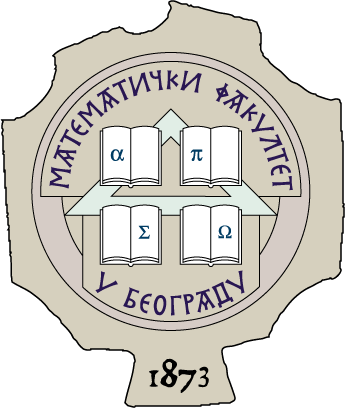
\includegraphics[scale=0.5]{images/grb.png}}
\end{figure}

\newpage

\renewcommand*\contentsname{\fontencoding{OT2}\selectfont Sadr\v{z}aj}

\tableofcontents

\newpage

\section{\fontencoding{OT2}\selectfont Uvod}
\textbf Segmentacija slika je jedan od najprostranjenijih na\v{c}ina za korektno klasifikovanje piksela u aplikacijama zasnovanim na odlu\v{c}ivanju. Segmentacija je tehnika koja particioni\v{s}e sliku na uniformne i nepreklapaju\'{c}e delove, zasnovano na nekoj meri sli\v{c}nosti. Ova tehnika ima veliki broj primena u analizi slika, medicinskom procesiranju slika, geografskom informacionom sistemu, i dr. Poslednjih godina, iskazano je veliko interesovanje za analizu slika, i s vremenom se ova oblast sve vi\v{s}e razvija. Na\v{s} rad se bavi problemom segmentacije slika kori\v{s}\'{c}enjem tehnike {\fontencoding{T1}\selectfont fuzzy} klasterovanja. Najvi\v{s}e pa\v{z}nje \'{c}e biti posve\'{c}eno problemu detekcije tumora na mozgu segmentovanjem rendgenskih snimaka.


\subsection{\fontencoding{OT2}\selectfont Definicija klasterovanja}

Ne postoji formalna definicija klasterovanja. \textbf{Klaster analiza} je pronala\v{z}enje grupa objekata takvih da su objekti u jednoj grupi me\dj usobno sli\v{c}niji u odnosu na objekte u razli\v{c}itim grupama. \textbf{Klasterovanje} se odnosi na postupak izdvajanja klastera. Problem klasterovanja se mo\v{z}e definisati na slede\'{c}i na\v{c}in: Dat je \v{z}eljeni broj klastera \textbf{\fontencoding{T1}\selectfont K}, skup podataka od \textbf{\fontencoding{T1}\selectfont N} ta\v{c}aka i funkcija za merenje rastojanja. Potrebno je prona\'ci particije skupa podataka tako da se minimizuje vrednost funkcije za merenje.

\subsection{\fontencoding{OT2}\selectfont Vrste klasterovanja}


\begin{itemize}

\item \textbf{Particiono klasterovanje}: Podela skupa podataka u nepreklapaju\'{c}e podskupove (klastere) takve da je svaki podatak ta\v{c}no u jednom podskupu.\\
\begin{figure}[h]
\fontencoding{OT2}\selectfont
\centerline{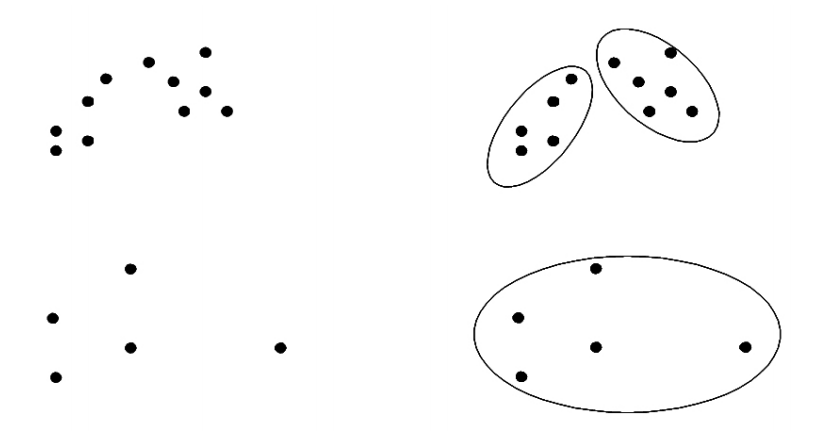
\includegraphics[scale=0.35]{images/part_klast.png}}
\caption{Levo - po\v{c}etni podaci. Desno - Particiono klasterovanje.}
\end{figure}
\item \textbf{Hijerarhijsko klasterovanje}: Skup ugnje\v{z}denih klastera organizovan u obliku hijerarhijskog stabla.
\begin{figure}[h]
\fontencoding{OT2}\selectfont
\centerline{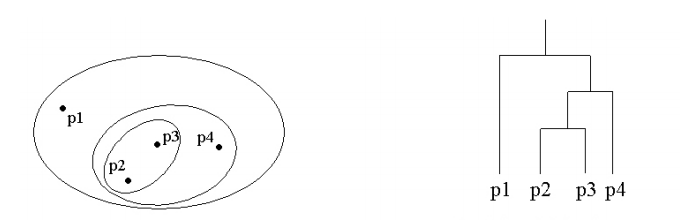
\includegraphics[scale=0.45]{images/hie_clast.png}}
\caption{Levo - hijerarhijsko klasterovanje. Desno - dengogram.}
\end{figure}

\end{itemize}

\subsection{\fontencoding{OT2}\selectfont Razli\v{c}iti tipovi klasterovanja}

\begin{itemize}
\item Ekskluzivno/neekskluzivno klasterovanje
\item {\fontencoding{T1}\selectfont Fuzzy} (rasplinuto/nerasplinuto) klasterovanje
\item Delimi\v{c}no/komplentno klasterovanje
\item Heterogeno/homogeno klasterovanje
\end{itemize}

\subsection{\fontencoding{T1}\selectfont Fuzzy \fontencoding{OT2}\selectfont klasterovanje}

Kod klasi\v{c}nog klasterovanja, podaci su podeljeni u odre\dj en broj disjunktnih klastera, gde jedan element mo\v{z}e pripadati samo jednom klasteru. U {\fontencoding{T1}\selectfont fuzzy} klasterovanju ta\v{c}ka mo\v{z}e pripadati ve\'{c}em broju klastera sa nekom te\v{z}inom izme\dj u 0 i 1. Zbir svih te\v{z}ina je jednak 1. Sli\v{c}ne karakteristike ima verovatnosno klasterovanje. {\fontencoding{T1}\selectfont Fuzzy} klasterovanje se jo\v{s} naziva i rasplinuto klasterovanje.


\section{\fontencoding{OT2}\selectfont Segmentacija slika}

Postoje mnogobrojne metode i raznovrsna literatura za izdvajanje informacija sa slike i njenu podelu na razli\v{c}ite regione. Svaka od tih metoda susre\'{c}e se sa odre\dj enim ograni\v{c}enjima koja se ogledaju u vremenskoj slo\v{z}enosti ili ta\v{c}nosti. Razlog za to je \v{s}to ne postoje jasne granice izme\dj u objekata na slici. {\fontencoding{T1}\selectfont Fuzzy} klasterovanje pokazalo se kao veoma dobar na\v{c}in za prevazila\v{z}enje ovog problema.

Segmentacija slika kori\v{s}\'{c}enjem {\fontencoding{T1}\selectfont fuzzy} klasterovanja bila je predmet velikog interesovanja kroz godine. Neki od algoritama koji se bave ovom temom su {\fontencoding{T1}\selectfont Fuzzy C-Means (FCM), Gustafson-Kesse (GK), Gaussian Mixture Decomposition (GMD), Fuzzy C-Varieties (FCV), Adaptive Fuzzy-C varieties (AFC), Fuzzy C-Shell (FCS), Fuzzy C-Spherical Shells (FCSS), Fuzzy C-Rings, Fuzzy C-Quadric Shells (FCQS), Fuzzy C- Rectangular Shells (FCRS)} i drugi. Me\dj u svim gore navedenim algoritmima, metod {\fontencoding{T1}\selectfont FCM}
je najprihva\'{c}eniji na\v{c}in za segmentaciju slika jer omogu\'{c}ava manji gubitak informacija u odnosu na algoritme klasi\v{c}nog klasterovanja. 


\subsection{\fontencoding{T1}\selectfont Fuzzy c-means}

{\fontencoding{T1}\selectfont Fuzzy c-means} je prvi put predstavio {\fontencoding{T1}\selectfont Dunn} a potom ga je modifikovao {\fontencoding{T1}\selectfont Bezdek}.

Sledi detaljan opis algoritma:

\begin{itemize}

\item Ulazni parametri: Podaci koje \v{z}elimo da klasterujemo (skup elemenata $x$ dimenizje $n$) i broj koji ozna\v{c}ava koliko klastera \v{z}elimo da dobijemo ($k$).
\item Izlazni paramteri: Matrica pripadnosti klasterima (dimenzije $n \times k$ ) i matrica centroida klastera(dimenzije $k \times d$ gde je $d$ dimenzija svakog pojedina\v{c}nog elementa iz skupa $x$).

\end{itemize}

Koraci algoritma:

\begin{enumerate}

\item Nasumi\v{c}no dodeljujemo vrednosti za sve te\v{z}ine u oznaci: $w_{ij}, \\ 1\leq i \leq n, \quad 1\leq i \leq n$ uz uslove:
\begin{enumerate}
\item $ \sum_{j=1}^k w_{ij} = 1, \quad \forall i\in {1,2,...,n}$
\item $ 0 < \sum_{i=1}^n w_{ij} < n, \quad \forall j\in {1,2,...,k} $
\end{enumerate}
\item Ra\v{c}unanje centroida za sve klastere u oznaci $c_j$ pomo\'{c}u formule:
\begin{equation}
c_j = \frac{\sum_{i=1}^n w_{ij}^p x_i}{\sum_{i=1}^n w_{ij}^p}
\end{equation}
Napomena: ako je $p = 0$, ima\'{c}emo pona\v{s}anje klasi\v{c}nog {\fontencoding{T1}\selectfont k-means} algoritma.
\item A\v{z}uriranje vrednosti matrice pripadnosti koriste\'{c}i formulu:
\begin{equation}
w_{ij} = \frac{\frac{1}{dist(x_i, c_j)}^\frac{1}{p-1}}{\sum_{q=1}^k \frac{1}{dist(x_i, c_q)}^\frac{1}{p-1}}
\end{equation}
\item Ponavljati korake 2. i 3. dok centroidi ne ostanu isti u dve iteracije za redom.

\end{enumerate}

Mera kvaliteta klasterovanja je suma kvadratne gre\v{s}ke(eng. {\fontencoding{T1}\selectfont Sum of Squared Error}):
\begin{equation}
SSE = \sum_{j=1}^k\sum_{i=1}^n w_{ij}^p dist(x_i, c_j), \quad p \in 1,...,\infty
\end{equation}

\subsubsection{\fontencoding{OT2}\selectfont Na\v{s}a implementacija algoritma {\fontencoding{T1}\selectfont fuzzy c-means}}

Re\v{s}enje problema segmentacije slika uz pomo\'{c} algoritma {\fontencoding{T1}\selectfont fuzzy c-means} smo implementirali u programskom jeziku {\fontencoding{T1}\selectfont Python}. Algoritam je implementiran u funkciji {\fontencoding{T1}\selectfont fuzzy\_c\_means}. Ona kao argumente prima:
\begin{itemize}
\item $data$ - niz podataka(to je ustvari matrica koja je dimenzije $n \times d$);
\item $n$ - ceo broj koji ozna\v{c}ava broj podataka koje \v{z}elimo da klasterujemo;
\item $k$ - ceo broj koji ozna\v{c}ava broj klastera;
\item $d$ - ceo broj koji ozna\v{c}ava dimenziju pojedina\v{c}nog podatka iz skupa podataka koje \v{z}elimo da klasterujemo;
\item $p$ - ceo broj koji ozna\v{c}ava paramear za {\fontencoding{T1}\selectfont fuzzy} formulu kojom odredjujemo stepen pripadnosti nekog podatka za svaki od klastera;
\item $max\_iter$ - ceo broj koji ozna\v{c}ava maksimalni broj iteracija zbog bezbednosti,
\end{itemize}
dok kao povratnu vrednost vra\'{c}a:
\begin{itemize} 
\item matricu $n \times k$ u kojoj \'{c}e element na poziciji biti $w_{ij}$, tj. te\v{z}ina sa kojom {\fontencoding{T1}\selectfont i}-ti element pripada {\fontencoding{T1}\selectfont j}-tom klasteru;
\item matricu $k \times d$ u kojoj \'{c}e se \v{c}uvati centroidi svih klastera.
\end{itemize}
Dakle, kako je jedna slika predstavljena kao matrica piksela gde je svaki piksel dimenzije 3, nju parsiramo u niz kako bismo je mogli, kao argument, proslediti na\v{s}oj funkciji. Nakon \v{s}to na\v{s}a funkcija kao povratnu vrednost vrati matricu pripadnosti podataka(u na\v{s}em slu\v{c}aju piksela dimenzije 3) klasterima svakom od piksela dodeljujemo vrednost centroida klastera za koji je vrednost najve\'ca u matrici pripadnosti. Zatim niz piksela vra\'{c}amo u matricu polaznih dimenzija i posmatramo je kao sliku. U na\v{s}em slu\v{c}aju vrlo je bitno da se jasno segmentuje odre\dj eni detalj na slici i zbog toga binarizujemo sliku, odnosno predstavljamo je sa samo dve boje.\\
{\fontencoding{T1}\selectfont Python} biblioteke kori\v{s}\'{c}ene u na\v{s}em re\v{s}enju su:
\fontencoding{T1}\selectfont
\begin{itemize}
\item numpy
\item matplotlib.pyplot
\item os
\item cv2
\item time
\item math
\end{itemize}
\fontencoding{OT2}\selectfont

\newpage

\subsubsection{\fontencoding{OT2}\selectfont Rezultati na\v{s}eg algoritma {\fontencoding{T1}\selectfont fuzzy c-means} na nekim rendgenskim snimcima tumora}



\begin{figure}[h]
\centerline{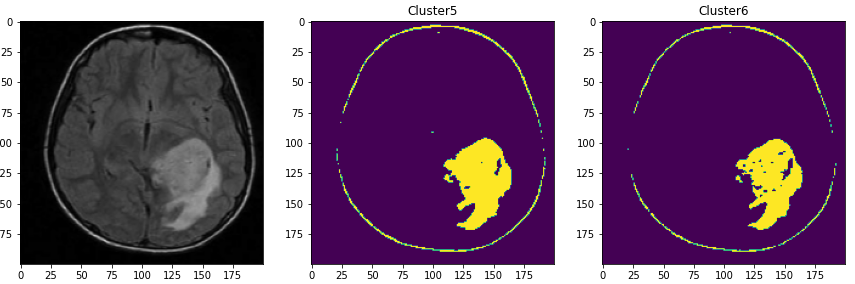
\includegraphics[scale=0.45]{images/segmented0.png}}
\centerline{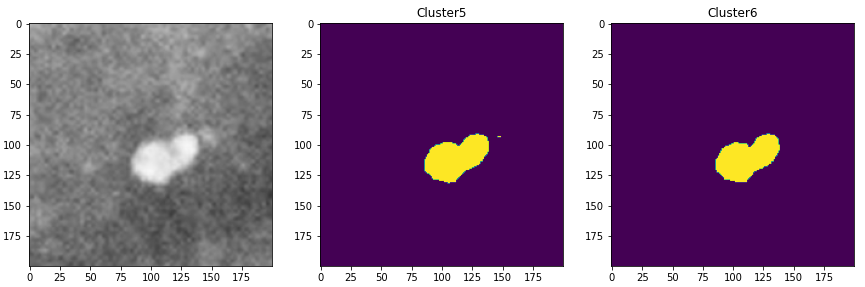
\includegraphics[scale=0.45]{images/segmented1.png}}
\centerline{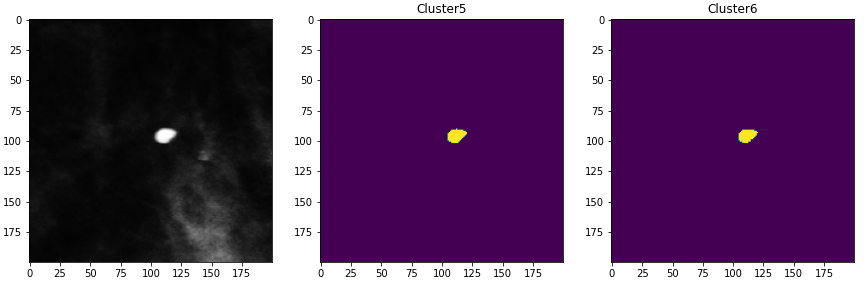
\includegraphics[scale=0.45]{images/segmented2.png}}
\end{figure}

\subsection{\fontencoding{T1}\selectfont K-means}

K-means algoritam je iterativni algoritam koji poku\v{s}ava podeliti skup podataka u K zasebnih podgrupa(klastera).

Sledi detaljan opis algoritma:

\begin{itemize}

\item Ulazni parametri: Podaci koje \v{z}elimo da klasterujemo (skup elemenata $x$ dimenizje $n$) i broj koji ozna\v{c}ava koliko klastera \v{z}elimo da dobijemo ($k$).
\item Izlazni paramteri: Matrica pripadnosti klasterima (dimenzije $n \times 2$ ) i matrica centroida klastera(dimenzije $k \times d$ gde je $d$ dimenzija svakog pojedina\v{c}nog elementa iz skupa $x$).

Koraci algoritma:

\begin{enumerate}

\item Navodimo \v{z}eljeni broj klastera.
\item Nasumi\v{c}no dodeljujemo vrednosti za centroide svih klastera u oznaci $c_j$. 
\item Ra\v{c}unanje centroida za sve klastere kao aritmeti\v{c}ke sredine svih elemenata u klasteru.
\item Za svaki podatak a\v{z}uriramo klaster kom on pripada tako da pripada klasteru \v{c}iji centroid mu je najbli\v{z}i.
\item Ponavljamo korake 2. i 3. dok centroidi ne ostanu isti u dve iteracije za redom.

\end{enumerate}

Mera kvaliteta klasterovanja je suma kvadratne gre\v{s}ke(eng. {\fontencoding{T1}\selectfont Sum of Squared Error}).

\subsubsection{\fontencoding{OT2}\selectfont Na\v{s}a implementacija algoritma {\fontencoding{T1}\selectfont k-means}}

Re\v{s}enje problema segmentacije slika uz pomo\'{c} algoritma {\fontencoding{T1}\selectfont k-means} smo implementirali u programskom jeziku {\fontencoding{T1}\selectfont Python}. Algoritam je implementiran u funkciji {\fontencoding{T1}\selectfont k\_means}. Ona kao argumente prima:
\begin{itemize}
\item $data$ - niz podataka(to je ustvari matrica koja je dimenzije $n \times d$);
\item $n$ - ceo broj koji ozna\v{c}ava broj podataka koje \v{z}elimo da klasterujemo;
\item $k$ - ceo broj koji ozna\v{c}ava broj klastera;
\item $d$ - ceo broj koji ozna\v{c}ava dimenziju pojedina\v{c}nog podatka iz skupa podataka koje \v{z}elimo da klasterujemo;
\item $max\_iter$ - ceo broj koji ozna\v{c}ava maksimalni broj iteracija zbog bezbednosti,
\end{itemize}
dok kao povratnu vrednost vra\'{c}a:
\begin{itemize} 
\item matricu $n \times 2$ u kojoj \'{c}e se uz element nalaziti oznaka klastera kom pripada;
\item matricu $k \times d$ u kojoj \'{c}e se \v{c}uvati centroidi svih klastera.
\end{itemize}
Dakle, kako je jedna slika predstavljena kao matrica piksela gde je svaki piksel dimenzije 3, nju parsiramo u niz kako bismo je mogli, kao argument, proslediti na\v{s}oj funkciji. Nakon \v{s}to na\v{s}a funkcija kao povratnu vrednost vrati matricu pripadnosti podataka(u na\v{s}em slu\v{c}aju piksela dimenzije 3) klasterima svakom od piksela dodeljujemo vrednost centroida klastera kom pripada. Zatim niz piksela vra\'{c}amo u matricu polaznih dimenzija i posmatramo je kao sliku. U na\v{s}em slu\v{c}aju vrlo je bitno da se jasno segmentuje odre\dj eni detalj na slici i zbog toga binarizujemo sliku, odnosno predstavljamo je sa samo dve boje.\\
{\fontencoding{T1}\selectfont Python} biblioteke kori\v{s}\'{c}ene u na\v{s}em re\v{s}enju su:
\fontencoding{T1}\selectfont
\begin{itemize}
\item numpy
\item matplotlib.pyplot
\item os
\item cv2
\item time
\item math
\end{itemize}
\fontencoding{OT2}\selectfont

\newpage

\subsubsection{\fontencoding{OT2}\selectfont Rezultati na\v{s}eg algoritma {\fontencoding{T1}\selectfont k-means} na nekim rendgenskim snimcima tumora}

\begin{figure}[h]
\centerline{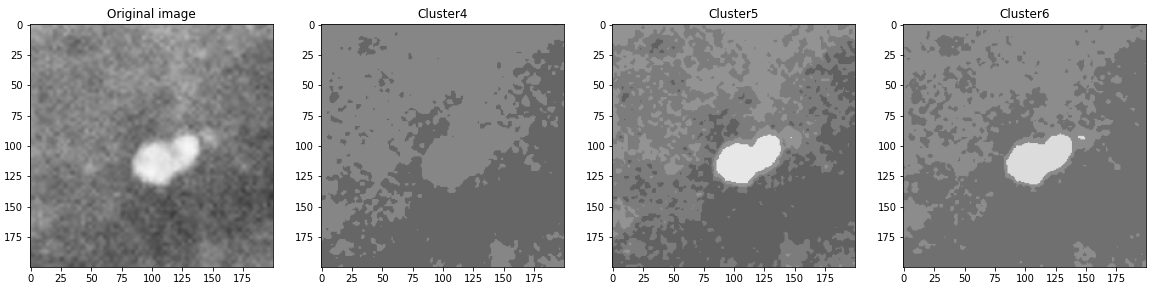
\includegraphics[scale=0.45]{images/segmented_k_means0.png}}
\centerline{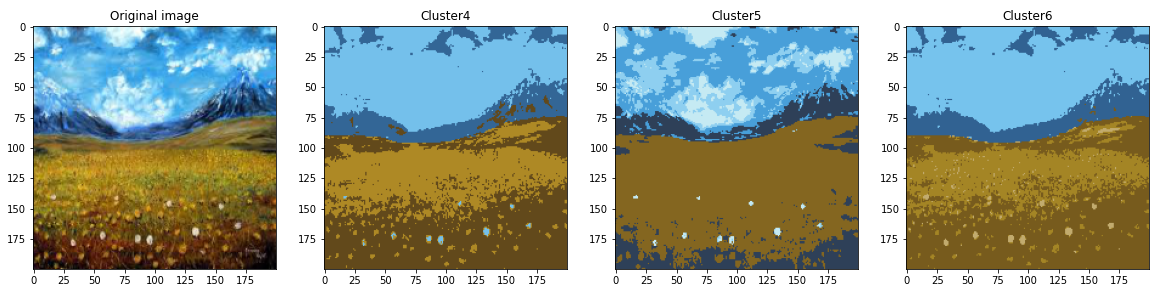
\includegraphics[scale=0.45]{images/segmented_k_means1.png}}
\centerline{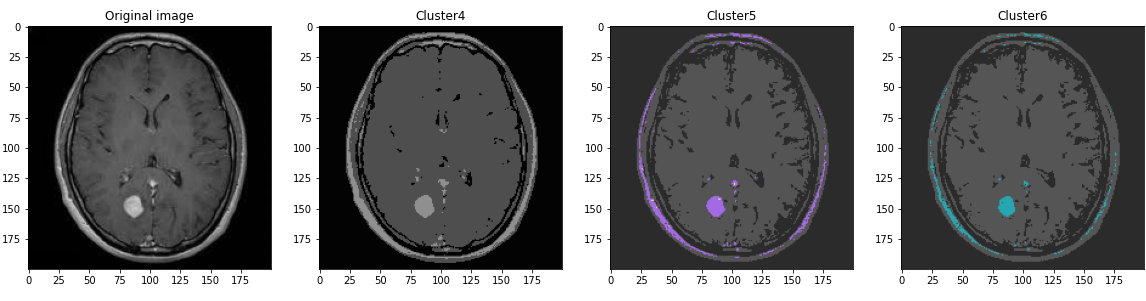
\includegraphics[scale=0.45]{images/segmented_k_means2.png}}
\end{figure}

\newpage

\end{itemize}

\section{\fontencoding{OT2}\selectfont Zaklju\v{c}ak}

Klasterovanje je jedan od najkori\v{s}\'{c}enijih na\v{c}ina za segmentaciju slika. Ogromna prednost {\fontencoding{T1}\selectfont fuzzy} klasterovanja u odnosu na ostale tehnike segmentacije slika je to \v{s}to je vrlo otporan na nepravilne granice. Tokom rada koristili smo vi\v{s}e razli\v{c}itih slika koje smo segmentovali uz isprobavanje razli\v{c}itih vrednosti odre\dj enih parametara i razli\v{c}itog broja klastera i u ve\'{c}ini slu\v{c}ajeva, kod {\fontencoding{T1}\selectfont fuzzy c-means} algoritma, najbolje se pokazalo kori\v{s}\'{c}enje 5 klastera uz parametar {\fontencoding{T1}\selectfont fuzzy} formule ($p$) koji je jednak 2, dok se kod {\fontencoding{T1}\selectfont k-means} algoritma ne mo\v{z}e jednostavno utvrditi za koji broj klastera daje najbolje rezultate s obzirom na to da smo u nekim situacijama pri radu sa eksperimentalnim podacima dobijali najbolju segmentaciju za jedan broj klastera, a onda kada bismo opet pokrenuli algoritam najbolja segmentacija bi se dobila za drugi broj klastera. Segmentacija slika uz pomo\'{c} algoritama {\fontencoding{T1}\selectfont fuzzy} klasterovanja je svoju primenu izme\dj u ostalog na\v{s}la u medicini gde je veoma bitna preciznost rezultata. Naravno, {\fontencoding{T1}\selectfont fuzzy} klasterovanje ima \v{s}irok spektar primene pored segmentacije slika u raznim drugim oblastima neke od njih su ekonomija, ve\v{s}ta\v{c}ka inteligencija i druge.

\subsection{\fontencoding{OT2}\selectfont Pore\dj enje rezultata}

Pore\dj enjem rezultata koje vra\'{c}aju algoritmi {\fontencoding{T1}\selectfont fuzzy c-means} i {\fontencoding{T1}\selectfont k-means} mo\v{z}emo videti da su slike primetno bolje segmentovane algoritmom {\fontencoding{T1}\selectfont fuzzy c-means}. Njegova slo\v{z}enost je ve\'{c}a od slo\v{z}enosti algoritma {\fontencoding{T1}\selectfont k-means} pa sam proces segmentacije traje ne\v{s}to du\v{z}e. Tako\dj e prednost algoritma {\fontencoding{T1}\selectfont fuzzy c-means} je to \v{s}to se u praksi pokazalo da daje skoro potpuno iste rezultate za isti broj klastera na istim slikama, dok kod algoritma {\fontencoding{T1}\selectfont k-means} to nije slu\v{c}aj.

\newpage
\section{\fontencoding{OT2}\selectfont Literatura}

\fontencoding{T1}\selectfont
\begin{itemize}
\item M.S. YANG - A Survey of Fuzzy Clustering, October 1993.
\item XL Xie, G Beni - A validity measure for fuzzy clustering, 1991.
\item Donald E. Gustafson, William C. Kessel - Fuzzy clustering with a fuzzy covariance matrix, 1979.
\item Imad Dabbura - K-means Clustering: Algorithm, Applications, Evaluation Methods, and Drawbacks, September 2018
\fontencoding{OT2}\selectfont
\item Mirjana Maljkovi\'{c} - Skalabilni klaster algoritmi, 2008.
\item Nenad Miti\'{c} - Predavanje o klaster analizi na Matemati\v{c}kom fakultetu, 2020.
\end{itemize}


\end{document}